\section{Discussion}\label{sec:discussion}

\subsection{Learning}\label{subsec:learning}
very cool! I tried spot checking different scans to see if I could tell the difference visually and I really really
cannot. I think it's encouraging that the model is able to notice impossible to visualize differences and run with it
this well. It's one thing to differentiate a st. bernard from a siamese cat, but two brain activations I'm not good at

\subsection{Future Works}\label{subsec:future-works}
Unsupervised segmentation, especially in 3d would be cool
Future works
- could strive to refine 3d more, with more time and compute
- unsupervised segmentation would be cool
- find ways to not have to smoosh images for memory?
- more visualizations? lack of color kinda sucks, saliency is weird, filters prob too

began work on visualization, it didn't lead anywhere useful, 1 channel might be a problem?
- check out filter viz
- see about unsupervised
- try 3d alternative archs? (dont really need to)

might want to improve 3d before going on to segmentation,
- scheduler / hyperparams / diff architectures (just go with res3d, res2d+1d, mix three types
wowee good stuff, hope to use a LR scheduler in the future to try to control this better?


 I'd be stoked
to reproduce on 3d, and trusting the model this much, open the door to segmentation

model ensemble (free extra few percent perf)
 \begin{figure}
  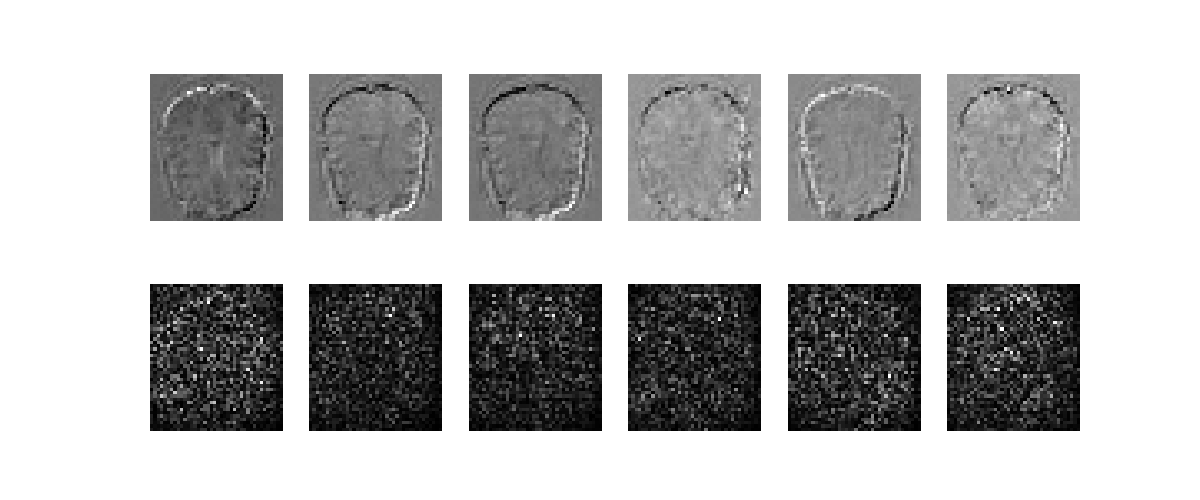
\includegraphics[width=\linewidth]{images/saliency.png}
  \caption{caption}
  \label{fig:saliency}
\end{figure}
